\newpage

\section{RISC-V: Compiling to a Modern RISC Architecture}

%\enquote{RISC-V is a recent, clean-slate, minimalist, and open ISA informed by mistakes of past ISAs. The goal of the RISC-V architects is for it to be effective for all computing devices, from the smallest to the fastest. Following von Neumann’s 70-year-old advice, this ISA emphasizes simplicity to keep costs low while having plenty of registers and transparent instruction speed to help compilers and assembly language programmers map actually important problems to appropriate, quick code.}\cite[p.~11]{Patterson2017}
% \begin{itemize}
% 	\item Introduced in 2011 X
% 	\item UC Berkely research project X
% 	\item Since then: rising in popularity X
% 	\item ISA = \enquote{instruction set architecture} X
% 	\item Was developed for: NO
% 	      \begin{itemize}
% 		      \item All sizes of processors: from embedded to high-performance computer
% 		      \item compatibility to popular software stacks and programming languages
% 		      \item serves as extendable base for customized accelerators
% 		      \item Should be stable
% 	      \end{itemize}
% 	\item One of the few ISAs which were developed this decade instead of the 1970s / 1980s X
% 	\item Open ISA: unlike most previous ISAs, it is free from a bond to a single comporation X
% 	\item Base ISA: \qVerb{RV321}.
% 	      Frozen, will never change, gives assembly programmers and compiler writers a stable target.
% 	\item The base instruction set is extendable using extensions like (multiply: \qVerb{RV32M}) or (double-precision floats: \qVerb{RV32D}).
% 	\item \enquote{RISC-V is a recent, clean-slate, minimalist, and open ISA informed by mistakes of past ISAs. The goal of the RISC-V architects is for it to be effective for all computing devices, from the smallest to the fastest. Following von Neumann’s 70-year-old advice, this ISA emphasizes simplicity to keep costs low while having plenty of registers and transparent instruction speed to help compilers and assembly language programmers map actually important problems to appropriate, quick code.}\cite[p.~11]{Patterson2017}
% \end{itemize} \cite[Chapter~1]{Patterson2017}.
%
% \TODO{Also interesting: \cite[p.~10]{Patterson2017}, \cite[Chapter~2]{Patterson2017}.}
%
% \begin{itemize}
% 	\item Present Some example instructions (Refer to chapter 3 of the RISC-V READER)
% 	\item Register layout \& count
% 	      RISC-V has 32 registers, ARM-32 16, x86\_32 has 8\\
% 	      Assembly includes all extensions\\
% 	      Concepts of \emph{pseudoinstructions}~\cite[p.~10]{Patterson2017}\\
% 	      Has basic instructions for add, sub, and logical operations\\
% 	      \emph{Check for all relationships between two registers, some conditional expressions involve rela- tionships between many pairs of registers. The compiler or assembly language programmer could use slt and the logical instructions and, or, xor to resolve more elaborate conditional expressions. The two remaining integer computation instructions Figure 2.1 help with assembly and}
% 	      r0 → constant 0 register\\
% 	      ~\cite[p.~18]{Patterson2017}
% 	\item ASM directives: \cite[p.~39]{Patterson2017}
% 	\item ASM includes 60 pseudoinstructions: \cite[p.~42]{Patterson2017}
% 	\item Another 32 Float registers, float load / store instructions: \cite[pp.~48f.]{Patterson2017}
% 	\item Refer to stack figure: \cite[p.~40]{Patterson2017}
% 	\item Calling convention
% \end{itemize}

The \emph{RISC-V} \emph{ISA}\footnote{Short for: \enquote{instruction set architecture}} is a new and modern \emph{reduced instruction set} architecture focussing on simplicity and expandability.
The initial version was developed at \emph{UC Berkely} in the context of another related research project.
Since its introduction in 2011, the architecture has been rapidly growing in popularity.
Since the beginning, the project has been managed and led by the \emph{RISC-V foundation}, consisting of many individuals contributing to the project.
Today, corporate members of the RISC-V foundation include companies like \emph{Google}, \emph{Microsoft}, \emph{Samsung}, and \emph{IBM}.
Therefore, the general popularity and commercial attraction of the technology is apparent.
However, unlike most previous ISAs, the RISC-V architecture is a completely \emph{open-source} project and is therefore not controlled by a single large corporate entity.
This can be regarded as a large competitive advantage over other popular RISC architectures like \emph{ARM}.
In the past, many ISAs have failed due to them being too restrictive with their licensing, thus preventing widespread commercial adoption.
However, RISC-V is completely open and free to use, so that many companies like \emph{Google} can leverage the technology commercially whilst contributing to the project.
Unlike most of the previous ISAs, which were developed during the 1970s or 80s, RISC-V is one of the few which were developed this decade.
Therefore, it seems like RISC-V could be a significant architecture to be used in all sorts of devices in the near future~\cite[preface]{Patterson2017}.

\subsection{Register Layout}

\begin{wraptable}{r}{.4\textwidth}
	\centering
	\caption{Common Registers in RISC-V~\cite[p.~155]{Waterman2019}}\label{tbl:riscv_regs}
	\begin{tabularx}{\linewidth}{l|L}
		\rowcolor{gray!10} Register   & Purpose                         \\ \hline
		\texttt{zero}                 & Hardwired zero                  \\ \hline
		\texttt{ra}                   & Return address                  \\ \hline
		\texttt{sp}                   & Stack pointer                   \\ \hline
		\texttt{t0} —  \texttt{t6}    & Temporary                       \\ \hline
		\texttt{fp}                   & Frame Pointer                   \\ \hline
		\texttt{a0}, \texttt{a1}      & Function argument, return value \\ \hline
		\texttt{a2} — \texttt{a7}     & Function argument               \\ \hline
		\texttt{s1} — \texttt{s11}    & Saved register                  \\ \hline
		\texttt{fa0}, \texttt{fa1}    & FP args, return value           \\ \hline
		\texttt{fa2} — \texttt{fa7}   & FP args                         \\ \hline
		\texttt{fs0} — \texttt{fs11}  & FP saved registers              \\ \hline
		\texttt{ft0} —  \texttt{ft11} & FP temporaries                  \\
	\end{tabularx}
\end{wraptable}

Most RISC architectures typically have a large count of registers~\cite[Chapter~2]{Dandamudi2005}.
When compared to other popular architectures, the truth of this statement becomes clear.
For instance, the \emph{x86\_32} architecture has 8 registers.
The popular RISC architecture \emph{ARM-32} provides twice that amount, meaning 16 registers.
However, a RISC-V CPU includes 32 registers, which is drastically more than the previously mentioned architectures.
Moreover, these 32 registers only include registers holding integer values.
Just for floating-point numbers, the ISA even provides another 32 registers.
Like previously explained, using more registers usually leads to increased efficiency of the output program.
Therefore, a register allocation algorithm targeting the RISC-V architecture could be more aggressive compared to one targeting x\_86 for instance~\cite[p.~10]{Patterson2017}.

The Table~\ref{tbl:riscv_regs} shows most of the registers which the RISC-V architecture provides.
For this table, the official ABI names of the registers have been used in order to make this section easier to read.
The first column of the table contains a register's name whilst the second column describes its purpose.

The first row of the table contains the \qVerb{zero} register.
On RISC-V, this register is special.
Like its name suggests, it holds the value of a constant 0.
Unlike other registers, it is read-only, meaning that it can never be overwritten, therefore preventing accidental writes.
In the next row, the \qVerb{ra} register is shown.
It saves the \emph{return address} of a function or subroutine.
If a return-instructions is used, the value in \qVerb{ra} is read as it is used to jump to a specific instruction.
The purpose of this register is elaborated further in Subsection~\ref{sec:riscv_calling_conv} about RISC-V's calling convention.
The \qVerb{sp} and \qVerb{fp} registers are used for managing stack memory.
Their purpose is explained in Subsection~\ref{sec:riscv_stack} about stack memory.
In the fourth row, the \qVerb{t0} — \qVerb{t6} are displayed.
These registers are often used to store temporary values used in larger computations.
In row six, the registers \qVerb{a0} and \qVerb{a1} can be seen.
These both serve as call arguments and return values of functions.
The remaining a-registers \qVerb{a2} — \qVerb{a7} can only be used as function call arguments.
How functions are called using registers will be explained in Subsection~\ref{sec:riscv_calling_conv}.
The next row contains the \emph{saved} registers \qVerb{s1} — \qVerb{s11}.
These registers are typically preserved across function calls, meaning a called function must not overwrite them.
However, this concept will also be explained in more detail later. \TODO{Will it?}
What the previously explained registers have in common is that they all hold integer values.
Depending on the exact RISC-V architecture, all registers either hold 32 or 64 bits of information.
For floating-point number values, RISC-V provides other registers.
Just like their integer counterparts, the floating-point registers \qVerb{fa0} and \qVerb{fa1} are used as function call arguments and as return values.
However, the other fa-registers \qVerb{fa2} — \qVerb{fa7} can only be used as function arguments holding floating-point numbers.
Just like the \qVerb{sx} registers, the \qVerb{fs0} — \qVerb{fs11} registers are usually preserved across function calls.
Last, the \qVerb{ft0} — \qVerb{ft11} registers can be used as temporary registers for floating-point numbers.
It is apparent that the floating-point registers are provisioned very similarly to the integer registers.
Therefore, a programmer or compiler targeting the architecture can utilize roughly the same principles,
regardless of the data-type stored in each register~\cite[pp.~18f,p.~34]{Patterson2017},~\cite[p~.155]{Waterman2019}.

Now, it has become apparent that RISC-V includes many registers which are grouped into semantic categories.
Every category is meant to be used in the specified manner, however, these groups are mostly only a suggestion of how each register should be used.
Although this subsection provides a good overview over the registers of the architecture, the purpose of some special registers is still not known.
These special registers, like \qVerb{sp}, \qVerb{fp}, and \qVerb{ra}, are thoroughly explained in the next sections.

\subsection{Memory Access Through the Stack}\label{sec:riscv_stack}

% \begin{wrapfigure}{R}{0.42\textwidth}
% 	\centering
% 	\begin{tikzpicture}[node distance=5mm]
% 		\node(stack)[
% 			vstack=6,
% 			rectangle split part fill={none, none, gray!20, gray!20, none, none},
% 			rectangle split part align=left,
% 		]{
% 			\nodepart{one}{{\texttt{\tiny 24(sp)}} fp$_0$}
% 			\nodepart{two}{{\texttt{\tiny 16(sp)}} ra$_0$}
% 			\nodepart{three}{{\texttt{\tiny -24(fp)}} \scriptsize a: int}
% 			\nodepart{four}{{\texttt{\tiny -25(sp)}} b: char}
% 			\nodepart{five}{{\texttt{\tiny 8(sp)}} fp$_1$}
% 			\nodepart{six}{{\texttt{\tiny 0(sp)}} ra$_1$}
% 		};
% 		\draw [thick, dashed] ([xshift=-.5cm, yshift=-.33cm]stack.four west) --  node[anchor=west, xshift=2cm, align=center] {\scriptsize function\\ \scriptsize boundary} ([xshift=.5cm, yshift=-.33cm]stack.four east);
%
% 		\node(sp)[left of=stack, xshift=-2.2cm, yshift=-0.32cm, align=left] {\scriptsize SP$_0$ \\ \scriptsize FP$_1$};
% 		\draw[arrow, shorten >= 2pt](sp) -- (stack.four west);
%
% 		\node(fp)[left of=stack, xshift=-2.2cm, yshift=2.26cm] {\scriptsize FP$_0$};
% 		\draw[arrow, shorten >= 2pt](fp) -- ([yshift=.74cm]stack.one west);
%
% 		\node(sp)[left of=stack, xshift=-2.2cm, yshift=-1.6cm] {\scriptsize SP$_1$};
% 		\draw[arrow, shorten >= 2pt](sp) -- (stack.six west);
% 	\end{tikzpicture}
% 	\caption{Spilled Registers During a RISC-V Function Call \TODO{Every row should be equal in height}}\label{fig:riscv_call_spill}
% \end{wrapfigure}

\begin{wrapfigure}{L}{0.39\textwidth}
	\hspace{-3.25cm}
	\begin{tikzpicture}[scale=.9]
		\small
		% TODO: also use longer arrow in top `fp_main`?
		\stackTopFixed{...} \cellcom{\scriptsize 32(sp)} \cellptr{\scriptsize \tt fp\,$_\text{main}$}
		\startframe
		\cell{fp} \cellcom{\scriptsize 24(sp)}
		\cell{ra} \cellcom{\scriptsize 16(sp)}
		\cell{a: int} \cellcom{\scriptsize -24(fp)} \cellptrA{\scriptsize \texttt{sp\,$_\text{main}$}}
		\cell{b: char} \cellcom{\scriptsize -25(fp)} \cellptrA{\scriptsize \texttt{fp\,$_\text{foo}$}}
		\finishframe{\tt main}
		\startframe
		\cell{fp} \cellcom{\scriptsize 8(sp)}
		\cell{ra} \cellcom{\scriptsize 0(sp)} \cellptrA{\scriptsize \texttt{sp\,$_\text{foo}$}}
		\finishframe{\tt foo}
		% TODO: uncomment the line below?
		%\stackbottom
	\end{tikzpicture}
	\caption{Example Stack Layout in RISC-V}\label{fig:riscv_basic_stack}
\end{wrapfigure}

As mentioned in the dedicated \TODO{(sub)} section about the stack, it presents a way to save data outside of registers.
This subsection explains special conventions followed when using stack memory on RISC-V.
Just like previously explained, most stacks are accessed through the specialized pointers.
On RISC-V, there is a \emph{stack pointer} which is saved in the \qVerb{sp} register.
Furthermore, the \qVerb{fp} register contains the \emph{frame pointer}.

Like most memory stacks, the RISC-V stack grows downwards, meaning it progresses into lower memory regions.
In the current implementation of the rush RISC-V compiler, the stack pointer points to the last legal memory cell of the current stack frame.
Therefore, \qVerb{sp} points on the cell with the lowest address of the current stack frame.
On the other hand, the frame pointer \qVerb{fp} points to the cell above the end of the current stack frame.
Therefore, the frame pointer always points to a memory cell which is illegal to use by the current function.
Thus, a stack frame is defined by its upper and lower bounds, represented by \qVerb{fp} and \qVerb{sp}, respectively.

In order to understand how the above behavior is used in practice, Figure~\ref{fig:riscv_basic_stack} is to be considered.
Furthermore, the rush program in Listing~\ref{lst:rush_riscv_stack} should be considered.

\Lirsting[caption={A rush Program Containing Two Variables}, label={lst:rush_riscv_stack}, float=H]{listings/riscv_stack.rush}

This snipped shows a rush program which contains two functions.
In the \qVerb{main} function of this program, two variables are defined.
The \qVerb{a} variable holds the integer value 42 whilst the \qVerb{b} variable contains the char value \qVerb{z}.
In line 4, the \qVerb{foo} function is called.
Figure~\ref{fig:riscv_basic_stack} shows the state of the stack at the point when this function was called.
The braces on the left side of the stack group the stack into frames.
On the right side of each stack cell, its relative address can be observed.
As explained previously, each stack cell is accessible either by offsetting \qVerb{sp}
or \qVerb{fp}. The stack pointers of each stack frame can are displayed by the arrows on the right side of the stack.

The stack shown in this figure contains two frames, one for each function involved in the call.
Since the \qVerb{main} function is called first, it is displayed at the top of the figure.
Normally, the last pushed element of a stack is located at the top, however, just as described,
this stack progresses towards lower memory, meaning that it grows downwards.
Since the \qVerb{main} function calls the \qVerb{foo} function, the stack frame for the \qVerb{foo} function is located at the bottom of the stack.

It is apparent that every stack frame saves the \qVerb{fp} and \qVerb{ra} registers at its top position.
These two special registers are saved at the two top positions of each call before any of the code in the function's body is executed.
Why these registers are saved on the stack is explained in Subsection~\ref{sec:riscv_stack} about the calling convention.
Since every stack frame contains these two elements,
the minimum size $s$ of a RISC-V stack frame in bytes must be $s = \frac{2 \times \text{Size}\,_\text{int}}{8}$.
Since $s$ is dependent on the integer-size of the RISC-V architecture, the minimum required memory differs per RISC-V architecture.
For instance, if the 64-bit version of RISC-V was used, the minimum size would be 16 bytes ($s = \frac{2 \times 64}{8} = 16$).
However, if the 32-bit version of the architecture was used, $s$ would be only 8 bytes ($s = \frac{2 \times 32}{8} = 8$).

Additionally, one can observe that the \qVerb{main} function's
stack frame contains cells which save the two variables which are defined in the body of the function.
Since the code in the function's body (where the variables are defined) is executed after \qVerb{fp} and \qVerb{ra} have been saved on the stack,
the cells containing these variables appear lower in the stack.
Another interesting observation is that the more recently declared variables are also saved in lower cells of the stack frame.
Therefore, the order in which variables are saved in the stack follows the \emph{LIFO} principle which is common in stacks.

In this example, in the stack frame of the function \qVerb{main}, the registers \qVerb{fp} and \qVerb{ra} require 16 bytes of memory together.
Therefore, the variable \qVerb{a} can be saved at the next 8 bytes of memory, meaning -24(fp).
This way, the variable is saved at the memory region from -24(fp) until the start of -16(fp) or 16(sp) in this example.
Therefore, each stack cell requires exactly as much memory as shown in the figure.
Just like described earlier, different rush types require different quantities of memory.
A character for instance only uses 1 byte of memory.
Thus, the entire variable \qVerb{b} is saved at -25(fp), meaning one byte below the end of the variable \qVerb{a}.
This way, each variable only uses as much memory as it actually requires.

However, the question of how the compiler is able to keep track of saved variables remains.
For this, the compiler maps a variable's name to a memory location.
To be precise, the compiler contains a \emph{HashMap} which associates a variable's name with its \qVerb{fp} offset.
In case of the program in Listing~\ref{lst:rush_riscv_stack}, the variable \qVerb{a} is associated with a \qVerb{fp} offset of -24.
If the variable is referenced at a later point, the compiler performs a simple lookup of the variable's memory address.

\TODO{How can we observe alignment here?}
\subsection{Calling Convention}\label{sec:riscv_calling_conv}

\TODO{did I mention that arguments are saved on the stack?}

\begin{wrapfigure}{R}{0.42\textwidth}
	\centering
	\begin{tikzpicture}[node distance=5mm]
		\node(stack)[
			vstack=6,
			rectangle split part fill={none, none, gray!20, gray!20, none, none},
			rectangle split part align=left,
		]{
			\nodepart{one}{{\texttt{\tiny 24(sp)}} fp$_0$}
			\nodepart{two}{{\texttt{\tiny 16(sp)}} ra$_0$}
			\nodepart{three}{{\texttt{\tiny 08(sp)}} argument 2}
			\nodepart{four}{{\texttt{\tiny 00(sp)}} argument 1}
			\nodepart{five}{{\texttt{\tiny 8(sp)}} fp$_1$}
			\nodepart{six}{{\texttt{\tiny 0(sp)}} ra$_1$}
		};
		\draw [thick, dashed] ([xshift=-.5cm, yshift=-.33cm]stack.four west) --  node[anchor=west, xshift=2cm, align=center] {\scriptsize function\\ \scriptsize boundary} ([xshift=.5cm, yshift=-.33cm]stack.four east);

		\node(sp)[left of=stack, xshift=-2.2cm, yshift=-0.32cm, align=left] {\scriptsize SP$_0$ \\ \scriptsize FP$_1$};
		\draw[arrow, shorten >= 2pt](sp) -- (stack.four west);

		\node(fp)[left of=stack, xshift=-2.2cm, yshift=2.26cm] {\scriptsize FP$_0$};
		\draw[arrow, shorten >= 2pt](fp) -- ([yshift=.74cm]stack.one west);

		\node(sp)[left of=stack, xshift=-2.2cm, yshift=-1.6cm] {\scriptsize SP$_1$};
		\draw[arrow, shorten >= 2pt](sp) -- (stack.six west);
	\end{tikzpicture}
	\caption{Spilled Registers During a RISC-V Function Call \TODO{Every row should be equal in height}}\label{fig:riscv_call_spill}
\end{wrapfigure}

Just like previously explained, most architectures provide a calling convention which dictates how low-level function calls should be managed.
For most architectures, the calling convention is part of the ISA's official specification.
In the case of RISC-V, the calling convention is specified in a separate document~\cite{RiscvABI2022}.

The first step of calling a function involves placing the arguments in a place where the function can access them.
For RISC-V, this involves placing the arguments into specialized registers.
Like described in the Table~\ref{tbl:riscv_regs}, only special classes of registers can be used as call arguments.
For integer arguments, the first arguments are placed in the registers \qVerb{a0}--\qVerb{a7}
For instance, the first two arguments of the rush function call
% TODO: this is broken? \LirstInline{rush}{let mut}
\qVerb{foo(40, 2, 3.14)} would be placed in the registers \qVerb{a0} and \qVerb{a1}.
However, the third argument is a floating-point number and can therefore not be placed inside an integer register.
Therefore, the first floating-point argument register \qVerb{fa0} contains the argument \qVerb{3.14}.
In this case, all arguments can be held in regisers and spilling would not be required.

In case the function accepted nine or more integer arguments,
all further integer arguments upward of the ninth position would have to be spilled on the stack.
Here, the successive registers \qVerb{a0}--\qVerb{a7} would contain the first eight integer arguments of the called function.
The argument at position 9 however is then spilled on the stack since there are no registers left which could contain the additional argument~\cite[p~.8]{RiscvABI2022}.

The Figure~\ref{fig:riscv_call_spill} displays a possible state of the call stack during a function call which uses ten integer arguments.
If ten integer arguments are used, two arguments would have to be spilled on the stack.
In the figure, the spilled registers are placed in the stack cells \enquote{argument 1} and \enquote{argument 2}.
Here, the cell \enquote{argument 1} would hold the ninth argument whilst \enquote{argument 2} holds the tenth argument.
Therefore, all spilled argument registers will be placed in the stack frame of the caller function.
Normally, variables saved on the stack are aligned to reflect their sizes.
In case of spilled argument registers however, every argument will occupy exactly 8 bytes on the stack, even if the data type itself requires less space.

Now that the first step of a procedure call is explained, the question of how the second step works in RISC-V remains.
In the second step, the underlying procedure call is made using a specialized instruction.
In RISC-V assembly, one typically uses the call \emph{pseudoinstruction}\footnote{A macro generating multiple instructions from one pseudoinstruction. Therefore, the actual count of ISA instructions remains low whilst convenience features can be used in assembly~\cite[p.~68]{Dandamudi2005}.}.
Due to a lack of functions in assembly, the call-instruction uses the name of its target label as one operand.
Therefore, labels can be called as if they were functions.
This instruction will jump to the first instruction of the specified target label whilst saving the address of the next instruction after the \qVerb{call} instruction in the register \qVerb{ra}~\cite[p.~22]{Patterson2017}.
As hinted previously, the \qVerb{ra} register saves the \emph{return address}.
Therefore, the return address is set every time a function call is performed.
% TODO: Since this register holds the address of the next instruction after the function's call-instruction, similarities to the call-stack of the rush VM can be noticed?

During the third step of the function call, the called function acquires local storage resources.
To be precise, the function decrements the stack pointer by the amount required by the stack frame.
Therefore, the function allocates as much stack space as required for storing local variables and other data.
Additionally, the frame pointer and return address are saved on the stack so that nested function calls do not cause issues.
For instance, if the return address was not saved on the stack, a nested function call would overwrite its stored value.
In this case, the parent function could no longer return since the return address now holds an incorrect value.
In order to mitigate issues like this, the return address and frame pointer are saved on the stack.
Figure~\ref{fig:riscv_call_spill} shows that the two registers are saved at the two positions on the top of the new stack frame.
This part of the function is often called the \emph{prologue} as it is executed before any of the function's internal code.

After the code of the function has been executed, the so-called \emph{epilogue} is executed.
Since the frame pointer and return address have been saved on the stack during the prologue,
the epilogue restores these registers by loading their values from the stack.
Furthermore, the amount which was subtracted from the stack pointer in the prologue is now added to the pointer in order to restore it to its original state before the function call.
Here, incrementing the stack pointer represents deallocating the previously acquired stack space.
However, the memory in the stack frame is not actually deleted since only the stack pointer is modified.
Even though the used memory is not explicitly deleted, it is still freed since it will probably be overwritten by the next function call.
If the prologue would not save the return address on the stack, a nested function call would overwrite the return address of the parent function, therefore creating a bug~\cite[p.33]{Patterson2017}.
By saving the return address on the stack, nested function calls do not cause difficulties.
It is apparent that this design contains a lot of similarities to the call-stack of the rush VM\@.
However, in the VM, the process of saving and restoring the return address was managed automatically by the VM,
whereas, here, the programmer has to manually pay attention to saving and restoring this important piece of data.
Therefore, implementing function calls is definitely more demanding in RISC-V assembly than in the rush VM\@.

In case a function returns a value, it must be communicated to the caller so that it can access it.
For integer-based types, the first return value of a function is placed in the register \qVerb{a0}
whilst floating-point numbers are placed in the register \qVerb{fa0}.
This way, the caller code can obtain a function's return value by accessing the \qVerb{a0} and \qVerb{fa0}
registers respectively. If a function does not return a value, these steps are just omitted.
It is to be mentioned that character and boolean values are also placed inside the \qVerb{a0} register since these types can be represented by integers.

Lastly, the epilogue contains a return-instruction which should jump to the place where the function was called.
This \emph{ret} instruction reads the value stored in \qVerb{ra} in order to jump to this address.


% \begin{figure}[h]
% 	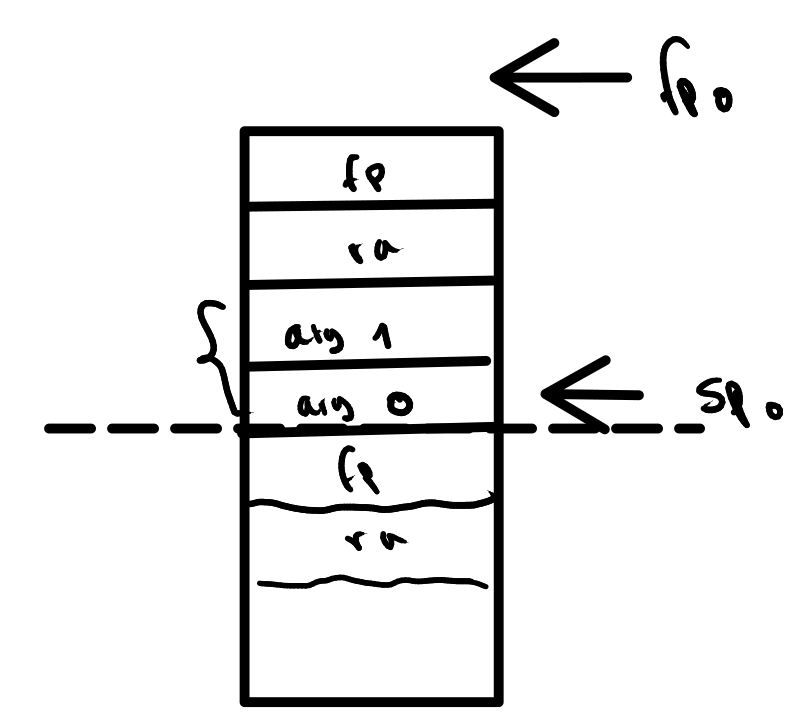
\includegraphics[width=.3\textwidth]{./riscv_call_stack_draft.png}
% 	\caption{\textcolor{red}{DRAFT:} Spilled Call Registers on the RISC-V Architecture}\label{fig:riscv_stack}
% \end{figure}

% \TODO{Continue here}
%
% \begin{itemize}
% 	\item Prologue
% 	      \begin{itemize}
% 		      \item Decrement stack pointer X
% 		      \item Adjust frame pointer    X
% 		      \item Save return address     X
% 	      \end{itemize}
% 	\item Epilogue
% 	      \begin{itemize}
% 		      \item Restore stack- and frame pointer X
% 		      \item Load previously saved return address X
% 		      \item Return to the caller instruction
% 	      \end{itemize}
% \end{itemize}
%

\subsection{The Core Library}

Like hinted in the section about the linker on page~\pageref{sec:linker},
a program might use functionality provided by external libraries.
In case of the rush RISC-V compiler, external functions are used for character-arithmetic,
the mathematical power operator, and \emph{kernel}\footnote{\TODO{Explaination + Citation}} system-calls,
like \emph{exit}\footnote{Terminates the execution of the program with an arbitrary exit code}.
Since these concepts must introduce additional logic, the compiler should not be emitted their instructions everytime they are used.
In that case, the repeated emission of redundant instructions would result in enlarged and unnecessary complex output code.
In order to mitigate these issues, the compiler simply inserts call-instructions referencing external functions.
External functions can be called just like any other function, however, their definition is not found in the same assembly file.
As described previously, resolving these external calls is later handled by the linker.
For this compiler, we later refer to this target specific library code by the term \emph{corelib}.

For instance, a function for mathematical power operations is implemented in the corelib.
Therefore, the compiler can emit a procedure call to this method every time rush's \qVerb{**} operator is used in the source program.
For this project, the entire corelib is written in RISC-V assembly.
However, it is often rational to implement a corelib or standardlib using a high-level language like C.
Since the corelib's functions are specified in separate files, they are packaged into an \emph{archive file}\footnote{\TODO{What are archives + Citation}} which is later used by the linker.

\subsection{RISC-V Assembly}

The Listing~\ref{lst:riscv_simple} shows a rush program containing two functions and a global variable.
In line 1 of the rush program, the mutable global variable \qVerb{m} is defined with the initial value 42.
In line 4 of the main-function, \qVerb{m} is incremented by 1.
Next, in line 5, the \qVerb{foo} function is called using \qVerb{m} as the only call argument.
\TODO{continue here}
In line 6, a return-statement is used to terminate the main-function explicitly.
The body of the \qVerb{foo} function only contains a call to the \qVerb{exit} function.
Therefore, the \qVerb{foo} function only exits using the specified parameter \qVerb{n} as the exit code.
In this case, the exit code of the displayed program will be 43.
The code in Listing~\ref{lst:riscv_simple_asm} on page~\pageref{lst:riscv_simple_asm} shows the output assembly generated from this program by the rush RISC-V compiler\footnote{Generated in Git commit \rushCommit, automatically built with this document}.
Because the assembler code of the \qVerb{foo} function would take up too much space in the assembler program, it is intentionally omitted from this listing.
Since the excluded function does not introduce any new concepts anyway, omitting it will not lead to a loss of explained concepts.

\Lirsting[float=H, caption={Example rush Program Containing Two Functions}, label={lst:riscv_simple}]{listings/riscv_simple.rush}

\begin{wrapfigure}{L}{0.5\textwidth}
	\centering
	\Lirsting[ranges={1-31, -4 53-56}, fancyvrb={frame=none}]{listings/generated/riscv_simple.s}
	\caption{Compiler Output from the Rush Program in Listing~\ref{lst:riscv_simple}}\label{lst:riscv_simple_asm}
\end{wrapfigure}

In line 1, the \qVerb{.global} assembler directive is used to declare the global symbol \qVerb{_start}~\cite[p~.36]{Patterson2017}.
On most architectures, the \qVerb{_start} label indicates a program's entry point, therefore marking the first instruction to be executed~\cite[p.~19]{Zhirkov2017-wk}.
In line 5, the \qVerb{_start} label is defined by placing a colon after its name.
In line 6, the \qVerb{call} instruction is used to call the \qVerb{main..main} function.
What strikes the eye here is that the already familiar \qVerb{main} function is prepended by the \qVerb{main..} prefix.
Since this rush compiler implements name mangling\footnote{Compilers often \emph{mangle} names in order to create a unique name for every function~\cite[pp.~119-120]{Levine2000}},
every function declared in a rush program will contain this prefix.
However, unlike high-level function calls in LLVM, this call instruction is used alongside the previously explained low-level calling conventions of RISC-V.

In the next line, the \qVerb{li} instruction is used to load the constant integer 0 into the register \qVerb{a0}~\cite[reference]{Patterson2017}.
Like explained in the previous section about the RISC-V calling convention,
the register \qVerb{a0} is used for the first integer call argument.
In line 8, the \qVerb{exit} function is called, however, one cannot see the definition of this function in the current file.
This is because the exit function is provided by the rush RISC-V corelib which was explained previously.
Since 0 was previously placed inside the register for the first integer call argument, the \qVerb{exit} function is called using 0 as the argument.
Therefore, the instructions in the lines 7--8 are responsible for terminating the program using the exit code 0.
These two instructions are always inserted at the end of the \qVerb{_start} label in order to terminate the program appropriately in case the rush code does not call \qVerb{exit} on its own.
This is required in order to prevent a segmentation fault which occurs if the program is not terminated properly.

Due to the function call in line 6, we will now shift our focus on the \qVerb{main..main} label in line 10.
In line 11, the first line of the \qVerb{main} function, a comment indicates the beginning of the function's prologue.
Just like demanded by the RISC-V calling convention, the rush compiler emits code for a \emph{prologue} and an \emph{epilogue} for each function.

As described in the previous sections about calling conventions, one task of the prologue is allocating stack space.
In this prologue, the \qVerb{addi} instruction in line 12 subtracts 16 from the value stored in \qVerb{sp}.
Since subtraction is used, the stack pointer is decremented, leading to the stack progressing into lower memory.
Therefore, this instruction increases the size of the stack, thus allocating memory.
Here, an addition instruction is used even though subtraction is required.
In RISC-V, the \qVerb{addi} instruction requires one register and one immediate value as its operands.
Due to the third operand being an \emph{immediate} value, the trailing \qVerb{i} (\emph{immediate}) appears in the instruction's name.
Since this immediate value can be negative, an additional instruction for immediate subtraction is redundant~\cite[reference]{Patterson2017}.
This example shows how the RISC-V ISA omits redundant instructions in places where it is feasible.
In this case, the stack pointer is decremented by 16 since two 8-byte values are stored on the stack in the lines 13 and 14.
Just like described in the previous subsection about the stack, these registers are always saved on the stack.

The comment in line 17 indicates the start of the function's body.
First, the previously explained \qVerb{li} instruction in line 18 places a constant 1 in register \qVerb{a0}.
Next, the \qVerb{ld} instruction in line 19 is used in order to load the value of the global variable \qVerb{m} into the register \qVerb{a0}~\cite[reference]{Patterson2017}.
Global variables, like \qVerb{m} in this example are saved under the \qVerb{.rodata}. section or under the \qVerb{.data} section if they are mutable.
In this example, \qVerb{m} is not declared as mutable and therefore saved under the \qVerb{.rodata} section.
The start of the \qVerb{.rodata} section is represented by the \qVerb{.section} assembler directive found in line 53.
Here, a label called \qVerb{m} is defined.
In this label, the \qVerb{.dword} directive is used to define the global initializer value of the variable.
In RISC-V, this directive stores 64 bit of information in successive memory doublewords~\cite[p.~39]{Patterson2017}.
The initializer value of the global variable is 42 and is represented as \qVerb{0x2a} using hexadecimal in the assembly code.
Since these data labels require their contents to be specified in hexadecimal, the trailing comment shows the base 10, human-readable version of the number.
Because global variable are not saved on the stack, special instructions like \qVerb{ld} are required to interact with global variables stored in the program's data sections.

At this point, the register \qVerb{a0} would contain 1 and \qVerb{a1} would contain 42.
In line 20, the \qVerb{add} instruction is used in order to save the sum of \qVerb{a0} and \qVerb{a1} in the register \qVerb{a2}.
Now, the value saved in \qVerb{a2} would be 43.
Next, the \qVerb{sd} instruction in line 21 saves the value of the register \qVerb{a2} at the memory location of the global variable \qVerb{m}, meaning that \qVerb{m} is updated to reflect its new value 43.
It now becomes apparent that these instructions are responsible for the add-assign expression in line 4 of the rush program.
Another interesting observation is that the last operand of the \qVerb{sd} instruction specifies the temporary register \qVerb{t6}.
The instruction uses this register for saving temporary data during the process of saving data in \qVerb{m}~\cite[reference]{Patterson2017}.

In line 22, the previously explained \qVerb{ld} instruction is used in order to load the value of the same variable into the register \qVerb{a0}.
Then, the \qVerb{call} instruction in line 23 is used in order to call the \qVerb{foo} function using the value of m as its argument.
However, one cannot easily observe how call arguments are passed here.
Like explained previously, the first integer argument of a function call must be placed in the register \qVerb{a0}.
Since \qVerb{m} was loaded into \qVerb{a0} previously, it will be used as the call argument for \qVerb{foo} automatically.
Therefore, the \qVerb{foo} function is called using 43 as the first argument.

Since the \qVerb{foo} instruction only calls the \qVerb{exit} function, its explanation will not be beneficial for introducing new concepts.
Therefore, we will omit the explanation of the assembler output of the \qVerb{foo} function.
The final instruction of the main-function's body is the \qVerb{j} instruction in line 24.
This instruction will cause the CPU to jump to the address of the specified label.
In this example, the CPU will jump to the first instruction of the \qVerb{epilogue_0} label~\cite[p.~17]{Patterson2017}.
Therefore, the rush compiler uses the \qVerb{call} instruction for jumps caused by function calls and the \qVerb{j} instruction for jumps between blocks of the current function.

Like explained previously, every function has a \emph{prologue} and an \emph{epilogue}.
Since one of the tasks handled by the epilogue is releasing resources allocated by the prologue, the function's stack pointer is incremented in line 30.
Finally, the \qVerb{ret} instruction in line 31 is used in order to jump back to the instruction whose address is specified in the \qVerb{ra} register~\cite[reference]{Patterson2017}.

\subsection{Supporting Pointers}

In Subsection~\ref{sec:pointers}, we have explained how pointers can be used in rush.
Since every rush backend should support all features of the language, pointers also need to be implemented for the RISC-V architecture.
In order to get a rough understanding of how pointers work in this compiler, the code in Listing~\ref{lst:rush_simple_pointer} and~\ref{lst:rush_simple_pointer_asm} are to be considered.

\begin{minipage}{.34\textwidth}
	\center
	\Lirsting[float=H, fancyvrb={frame=none}, caption={Example rush Program Containing a Pointer}, label={lst:rush_simple_pointer}]{listings/rush_simple_pointer.rush}
\end{minipage}%
\hspace{3cm}
\begin{minipage}{.45\textwidth}
	\center
	\Lirsting[float=H, fancyvrb={frame=none}, ranges={10-10,18-24}, caption={RISC-V Assembly Output from Listing~\ref{lst:rush_simple_pointer}}, label={lst:rush_simple_pointer_asm}]{listings/generated/riscv_rush_simple_pointer.s}
\end{minipage}


The code in Listing~\ref{lst:rush_simple_pointer} shows a rush program in which a variable is referenced to create a pointer which is then dereferenced.
In line 2, the mutable variable \qVerb{a} is defined using an initial value of 42.
Next, in line 3, the variable is referenced in order to use the resulting address to define the variable \qVerb{to_a}.
In line 4, the \qVerb{to_a} pointer variable is dereferenced in order to use the value of \qVerb{a} as the exit code of the program.


Listing~\ref{lst:rush_simple_pointer_asm} includes the most significant part of the compiler output which represents this rush program\footnote{Generated in Git commit \rushCommit, automatically built with this document}.
In line 18 of this listing, the integer value 42 is placed in the register \qVerb{a0}.
Next, \qVerb{a0} is saved on the stack at \qVerb{-24(fp)} using the \qVerb{sd} instruction.
Like the comment suggests, the instruction in line 20 is used in order to reference a.
Here, the \qVerb{addi} instruction is used to subtract 24 from the value stored in the \qVerb{fp} register.
The result of this subtraction is saved in the register \qVerb{a0}.
Therefore, the register now contains the absolute memory address of the \qVerb{a} variable.
Since the syntax \qVerb{-24(fp)} means that the variable is saved at $fp - 24$, the subtraction uses the exact same information which is already known about the variable.
Here, instead of using the saved memory location of the variable like \qVerb{x(fp)}, the information is used in order to calculate the absolute address of the target variable.
This computation can only be performed at runtime since the value of \qVerb{fp} is not known at compile time.
In line 21, the \qVerb{a0} register which contains the memory address is also saved on the stack.
Therefore, the \qVerb{a} variable is saved at \qVerb{-24(fp)} whilst \qVerb{to_a} is saved at \qVerb{-32(fp)}.

In order to access the value of \qVerb{a}, \qVerb{to_a} is dereferenced in line 4 of the rush program.
For this, the memory address stored in the variable \qVerb{to_a} first needs to be loaded from the stack.
Here, the \qVerb{ld} instruction in line 22 of the assembly output is used.
The instruction will load the memory address stored at \qVerb{-32(fp)} (in \qVerb{to_a}) into the \qVerb{a0} register.
Next, another \qVerb{ld} instruction in line 23 is used in order to load the value of the variable saved at the previously fetched memory address.
What strikes the eye is that \qVerb{0(a0)} instead of \qVerb{x(fp)} is used for specifying the target memory address of the load instruction.
In this case, \qVerb{0(a0)} means that the instruction should load its value from the address saved in \qVerb{a0} with an offset of 0.
Since an offset of 0 is used, the practical description of the instruction is that it loads a value saved at the memory address specified in \qVerb{a0}.
Because \qVerb{a0} contains the memory address of the \qVerb{a} variable, the instruction loads 42 into the \qVerb{a0} register.

\subsection{The rush Compiler Targeting RISC-V Assembly}

Just like the other compilers presented in this paper, this one also traverses the annotated AST using the postorder technique.
Unlike the LLVM or WASM compiler, this compiler emits RISC-V assembly files which are later assembled by the assembler.

\subsubsection{Struct Fields}

Before any complex code samples can be considered, important struct fields of the compiler first need to be explained.
The rust code in Listing~\ref{lst:riscv_compiler_attr} shows important struct fields of the rush compiler targeting RISC-V.

\Lirsting[ranges={11-11,15-15,19-34}, caption={Fields of the RISC-V \qVerb{Compiler} Struct}, label={lst:riscv_compiler_attr}, float=H]{deps/rush/crates/rush-compiler-risc-v/src/compiler.rs}

In line 15, the field \qVerb{blocks} is declared.
This field holds a vector containing values of the type \qVerb{Block}.
That type provides an abstraction representing a label with its basic block in the assembly output.
Therefore, this struct needs to contain a string field for its label and a vector for its instructions.
The Listing~\ref{lst:riscv_instruction_enum} shows parts of the Rust code which declares the \qVerb{Instruction} enum.

\Lirsting[ranges={62-62,74-76,114-114}, caption={The \qVerb{Instruction} Enum in the RISC-V Compiler}, label={lst:riscv_instruction_enum}, float=H]{deps/rush/crates/rush-compiler-risc-v/src/instruction.rs}

Although the listing shows only a few of the implemented instructions, this enum contains all instruction variants which the compiler might need at a later point.
Depending on the type of instruction, the corresponding enum includes fields which define its operands.
For instance, the \qVerb{Li} variant in line 74 represents the \qVerb{li} instruction in assembly.
This instruction loads the immediate integer value specified in the second operand into the register specified in the first operand.
Due to this, the enum also contains a field for a value of the type \qVerb{IntRegister} and a field for a 64-bit signed integer.
The Rust code in Listing~\ref{lst:riscv_intregister_enum} shows parts of the declaration of the \qVerb{IntRegister} enum.
Like the name implies, this enum holds all possible registers which the architecture provides.

\Lirsting[ranges={107-107,137-139,145-145}, caption={The \qVerb{IntRegister} Enum in the RISC-V Compiler}, label={lst:riscv_intregister_enum}, float=H]{deps/rush/crates/rush-compiler-risc-v/src/register.rs}

Even though just the integer registers are shown in this listing, a similar enum for floating-point registers also exists in this implementation.
Another important struct field is declared in line 19 of Listing~\ref{lst:riscv_compiler_attr}.
The \qVerb{curr_block} field saves the index of the basic block which is currently being inserted to.
Next, the \qVerb{data_section} and \qVerb{rodata_section} fields in line 21 and 22 are declared.
Just like the ELF sections, these vectors contain declarations of global variables in the program.
Here, each vector holds items of the type \qVerb{DataObj}.
Since this type specifies data which should be saved in these sections, it contains a string field for the label and an enum field for the actual data saved in the object.
For instance, if the compiler encounters a global variable declaration, a new data object is inserted into the correct section, depending on whether the global variable has been declared as mutable or not.

In line 25, the \qVerb{curr_fn} field is declared.
This field saves a value of the type \qVerb{Function}.
The \qVerb{Function} struct contains a counter of the stack allocations of the current function in bytes and the label of the epilogue block of the current function.
The former is incremented every time a variable declaration is compiled.
This is required in order to allocate the correct amount of stack memory during a function's prologue.
\TODO{describe let and prologue later}

Just like in the other compilers, this one also features a \qVerb{loops} field which saves important labels of the current loop being compiled.
This field is declared in line 27 and holds a vector of \qVerb{Loop} structs.
Each \qVerb{Loop} struct saves the label of the loop's head and the label of the basic block which follows after the loop's body.
\TODO{Explain loop labels later}

Furthermore, the \qVerb{scopes} field in line 29 is managed to associate a variable to some important metadata.
This metadata includes the variables type and its \emph{stack memory position}.
Just like explained in the previous sections, each cell of the stack memory is accessible by specifying a unique index.
The compiler saves this unique index in this HashMap so that it can refer back to the variable later.
Of course, this only works for variables which are saved on the stack.
However, these HashMaps are not used for saving global variables.
Instead, the \qVerb{globals} field in line 31 is used.
Just like the HashMaps in the \qVerb{scopes} field, this map also associates a variable's name to a value of the type \qVerb{Variable}.
This time however, each variable contains the data label under which the global variable was declared.
Last, the \qVerb{used_registers} field in line 33 is declared.
It plays a vital role in the compiler's register allocation algorithm.

By only considering the compiler's struct fields, it has become apparent that this implementation provides several abstractions over the bare strings in which assembly is normally formatted.
Due to this, implementation of the actual compiler is a lot more structured and reliable.
During development of the compiler, this approach has often proven itself to be optimal.

\subsubsection{Data Flow and Register Allocation}

An important characteristic of a compiler is how it represents runtime data at compile time.
In assembly, runtime data is represented by registers which will contain values at runtime.
Since this rush compiler emits RISC-V assembly, it also represents data by using registers internally.
In the previous paragraphs, we have learned how this implementation uses abstractions in order to represent assembly constructs, including registers.

For reference, the LLVM compiler represents runtime values by passing virtual registers internally.
Similarly, this compiler also passes abstractions representing registers in order to represent the data flow of the program being compiled.
Unlike in LLVM, there is only a finite amount of registers available.
Therefore, this compiler also manages register allocation so that programs can be represented using this limited number of registers.
In under to understand the implementation, the code in Listing~\ref{lst:rush_riscv_simple_sum} and Listing~\ref{lst:rush_riscv_simple_sum} is to be considered.
The former listing contains a rush program which adds two integer variables together in order to use the result as its exit code.
The latter shows parts of the assembly output representing the logic in the \qVerb{main} function.

\begin{minipage}{.34\textwidth}
	\center
	\Lirsting[caption={Rush Program Calculating the Sum of Integers}, label={lst:rush_riscv_simple_sum}, float=H]{listings/simple_add.rush}
\end{minipage}%
\hspace{3cm}
\begin{minipage}{.45\textwidth}
	\center
	\Lirsting[ranges={18-25},caption={Assembly Output of Rush Program in Listing~\ref{lst:rush_riscv_simple_sum}}, label={lst:asm_riscv_simple_sum}, float=H]{listings/generated/rush_simple_add.s}
\end{minipage}

In the lines 2 and 3 of the rush program, the integer variables \qVerb{a} and \qVerb{b} are declared.
In line 4, the \qVerb{exit} function is invoked, using the sum of these variables as the call argument.

In the line 22 of the assembly output, the runtime value of the \qVerb{a} variable is loaded into the register \qVerb{a0}.
Next, the same operation is performed for the \qVerb{b} variable.
However, this time, the instruction writes its result in the \qVerb{a1} register instead of the \qVerb{a0} register.
This is because the previously loaded value in \qVerb{a0} would be overwritten if this was the case.
Since both the value of the variable \qVerb{a} and \qVerb{b} are required for the addition, overwriting this register would result in a wrong calculation.
This is am example of how register allocation is required in order to manage registers and to prevent such bugs.

Unlike the register allocation algorithm of a production ready compiler like LLVM, this one only aims to use registers without causing conflicts like the previously explained one.
Therefore, this algorithm does not emphasize performance and instead only performs mandatory task which are required for making a program work.
For instance, all variables are saved on the stack in order to keep all registers unused and free for use in temporary calculations and operations like this one.
Since this algorithm only performs rudimentary register allocation, its implementation is also significantly easier.

The core principle of the register allocator is that each method which can return a register decides which register it returns itself.
In order to choose an output register, each of those methods uses the helper method \qVerb{alloc_ireg}.
The rust code in Listing~\ref{lst:riscv_alloc_ireg} shows the \qVerb{alloc_ireg} method of the RISC-V rush compiler.

\Lirsting[ranges={175-186}, path prefix={deps/rush}, float=h, label={lst:riscv_alloc_ireg}, caption={\qVerb{alloc_ireg} Method of the RISC-V rush Compiler}]{deps/rush/crates/rush-compiler-risc-v/src/utils.rs}

This method returns the first available register from the register pool containing either integer registers\footnote{The \enquote{i} in \qVerb{alloc_ireg} hints that it allocates integer registers}.
Such a register pool contains all possible registers which can hold the data type of that class of registers.
This compiler contains two pools: one for integer registers and one for floating-point registers.
In line 175 of Listing~\ref{lst:riscv_alloc_ireg}, the signature of the method is shown.
Here, one can see that the method returns a value of type \qVerb{IntRegister}.
The for-loop in line 176 is used to itrate through the entire \qVerb{INT_REGISTERS} array.
This array is constant and therefore represents the pool containing integer registers.
In the lines 177--180, the if-expression checks if the current register (\qVerb{reg}) is not found in the \qVerb{used_registers} vector.
If this was the case, the current register would be unused and could therefore be returned.
Since the return-statement in line 182 returns the current register if it is unused, the loop only runs until a free register has been found.
Due to the passive nature of the register allocation algorithm used in this compiler, the unreachable-macro in line 185 should never be called since the compiler should not run out of registers.
However, one can see that this method does not mark the newly returned register as used.
This is because marking a register as used is only required in some sections of the compiler where overwriting a register would introduce a bug in the output program.
Therefore, if this method was to be called repeatedly without calls to other methods, it would always yield the same result register.

In order to mark a register as used, it is simply pushed into the \qVerb{used_registers} vector.
For this, a helper method called \qVerb{use_reg} which only performs this simple call is implemented.
Due to the simplicity of this method, a listing of its code is intentionally omitted.
If a register is no longer used and can be overwritten again, it is also simply removed from the \qVerb{used_registers} vector.
For this, another simple helper method called \qVerb{release_reg} is implemented.

\TODO{insert graphic}\\
\TODO{explain when registers are marked as used}

\begin{figure}
	\centering
	\begin{tikzpicture}
        \node(stack)[stack=6, rectangle split part align=center,
			rectangle split part fill={gray!20, gray!20, none, none, none, none},
            text width=10ex, text centered, inner xsep=0]{
            \shortstack{used\\\\\texttt{a0}}
            \nodepart{two}{\shortstack{used\\\\\texttt{a1}}}
            \nodepart{three}{\shortstack{unused\\\\\texttt{a2}}}
			\nodepart{four}{\ldots}
            \nodepart{five}{\shortstack{unused\\\\\texttt{a7}}}
			\nodepart{six}{\ldots}
		};
		\node(ff)[below of=stack, yshift=-.5cm] {\scriptsize first free};
		\draw[arrow, shorten >= 4pt](ff) -- (stack.three south);
	\end{tikzpicture}
	\caption{Integer Register Pool of the RISC-V rush Compiler}\label{fig:riscv_iregister_pool}
\end{figure}

Figure~\ref{fig:riscv_iregister_pool} shows an abstract representation of the compiler's integer register pool.
Here, the pool contains all integer registers of the compiler.
In this figure, only the first section of the pool which contains the \qVerb{ax} registers can be seen.
The gray cells at the beginning indicate that these registers are currently in use by the compiler.
Of course, this information is not saved in the register pool since the \qVerb{used_registers} vector saves this data.
In the figure, the arrow points to the first free register, meaning the one which follows the last used register \qVerb{a1}.
Therefore, if the \qVerb{alloc_ireg} method was called when the state of the registers is equivalent to the one displayed in Figure~\ref{fig:riscv_iregister_pool}, it would return the register \qVerb{a2}.
By considering this example, it has become apparent that the method always returns the first free integer register.
In the compiler, an equivalent pool for float registers also exists.

However, we still do not know when the compiler marks certain registers as used.
In order to understand this problem, the compilation of the rush expression \LirstInline{rush}{n + m} is to be considered.

\TODO{insert listing of infix compilation}

\begin{itemize}
	\item If a register cannot be overwritten, mark it as \enquote{used} X
	\item Each function decides which target register will hold its result X
	\item Registers are acquired from a pool of registers X
	\item the first free register from this pool is taken when a new register is requested X
	\item For instance, a new integer register can be acquired by calling the \qVerb{self.alloc_ireg} method. X
	\item If this function is called repeatedly, it would always return the same register, \qVerb{a0} for instance. X
	\item Therefore, registers can be marked as \qVerb{used}. X
	\item In this case, the method would return the next free register after the last used one X
	\item \TODO{include graphic here}
	\item Such a pool exists for both integer and floating-point registers X
	\item Include rust code which calls the \qVerb{alloc_ireg} and \qVerb{use_reg} methods (in the \qVerb{infix_expr} method) X
	\item The latter inserts a register into the \qVerb{used_registers} vector in order to block it temporarely
	\item Show code of the \qVerb{alloc_ireg} method and explain how it works and why it works like this
\end{itemize}

\begin{itemize}
	\item Traverses the tree X
	\item Show struct fields X
	\item Explain register allocation and flow of expressions / values
	\item Explain functions
	\item Explain let statements
	\item Explain calls
	\item Explain loops
	\item Explain floats
\end{itemize}
